\section{Data analysis}
Used dataset includes titles from links to articles on Twitter~\cite{ClickbaitDataset2016}. 
Online news media usually use Twitter to publish their links to attract users to their news website.

Human evaluators were employed to assign a clickbait score to
each tweet. They had four following options for each tweet:
\begin{itemize}
    \item $0$: not clickbaiting (option 1);
    \item $0.33$: slightly clickbaiting (option 2);
    \item $0.66$: considerably clickbaiting (option 3);
    \item $1$: clickbait (option 4).
\end{itemize}

\begin{figure}[H]
    \centering
    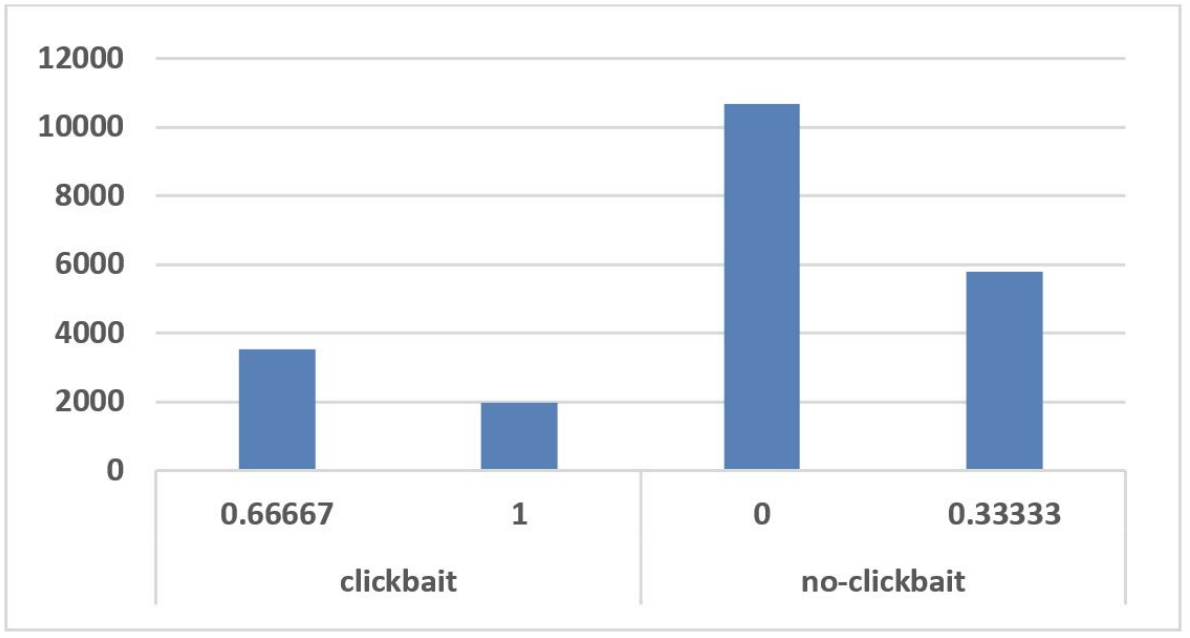
\includegraphics[width=0.75\textwidth]{data_label_median}
    \caption{Total count of tweets based on the median of the tweets’ scores for each binary label}
    \label{fig:data_label_median}
\end{figure}

As we can see on the figure~\ref{fig:data_label_median}, all the tweets that their median judgment score is 1 or 0.66667 are in the clickbait category. 
In contrast, those their median judgment score is 0 or 0.33333 are in
the non-clickbait category. So, we can conclude that if the sum of
selected <<slightly clickbaiting>> and <<not clickbaiting>> options is
bigger than the sum of two other options, the tweet will be labeled
as non-clickbait. Otherwise, it would be considered a clickbait.

So, for determining the label of the tweets, there is no difference
between the option 1 and the option 2 (i.e. <<not clickbaiting>> and <<slightly clickbaiting>>). Also, there is no difference between the option 3 and the option 4 (i.e. <<considerably clickbaiting>> and <<clickbait>>) as well.

\begin{figure}[H]
    \centering
    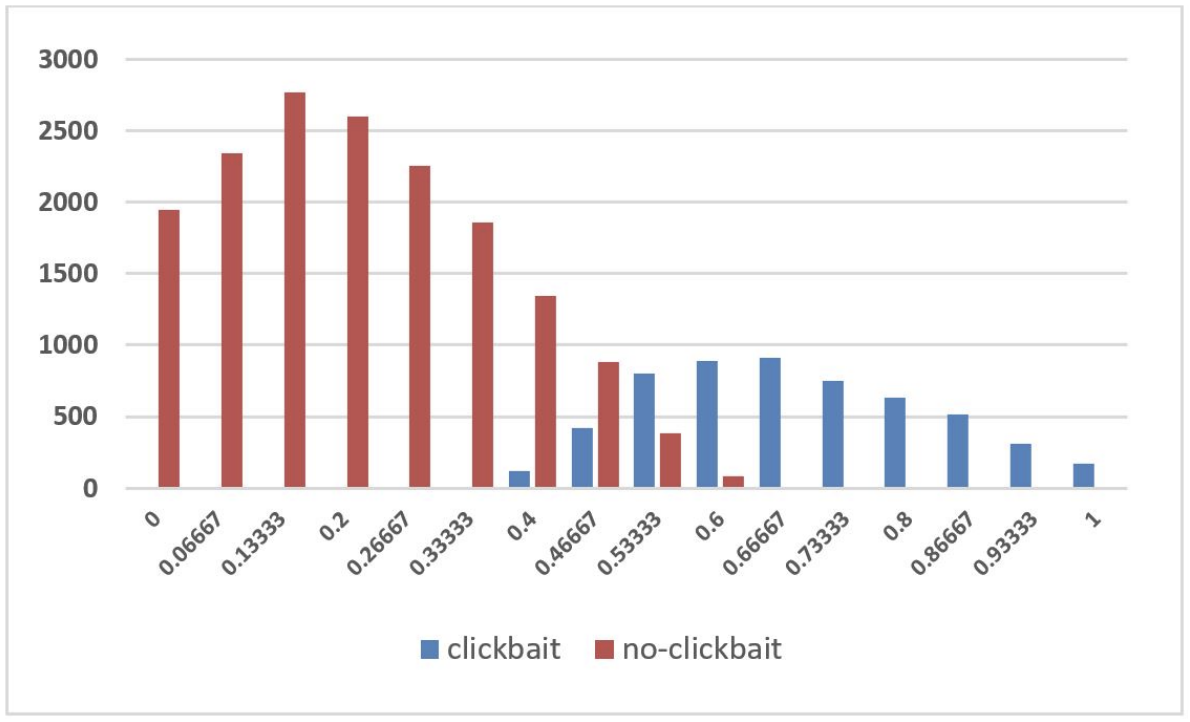
\includegraphics[width=0.75\textwidth]{data_label_distribution}
    \caption{Distribution of clickbait and non-clickbait tweets based on mean judgment score}
    \label{fig:data_label_distribution}
\end{figure}

Figure~\ref{fig:data_label_distribution} shows the distribution of mean judgment score for the tweets in both clickbait and non-clickbait categories. It can be seen how clickbait and non-clickbait tweets have overlap between 0.4 and 0.6 values in terms of mean judgment score.

\begin{figure}[H]
    \centering
    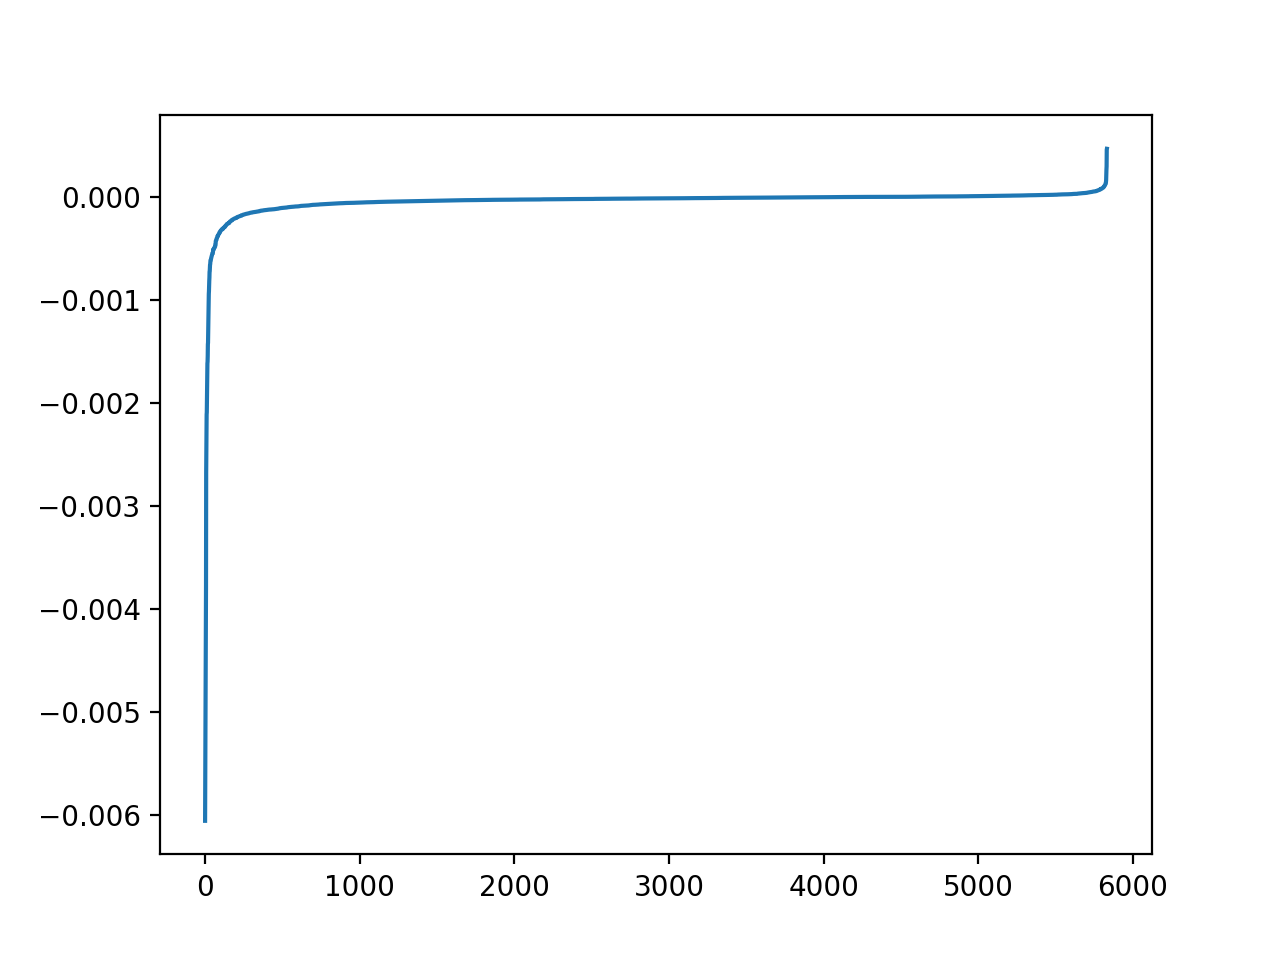
\includegraphics[width=0.75\textwidth]{data_freq}
    \caption{Distribution of clickbait and non-clickbait words in dataset}
    \label{fig:data_freq}
\end{figure}

Figure~\ref{fig:data_freq} shows the distribution of words in both clickbait and non-clickbait categories (word is classified as a clickbait if more frequently used in clickbait titles and vice versa; positive score represents clickbait words). It can be seen that some words have strong relation to the clickbait score.